\documentclass[11pt]{article}

\usepackage[paperheight=8in, paperwidth=6in, 
  hmargin=0.25in, vmargin=0.25in]{geometry}

\usepackage[T1]{fontenc}
\usepackage{libertinus}
\usepackage{libertinust1math}
\usepackage{inconsolata}

\usepackage{titlesec}
\titleformat{\section}{\normalfont\sffamily\bfseries}{\thesection}{1em}{}
\titleformat{\subsection}{\normalfont\sffamily}{\thesubsection}{1em}{}

\usepackage{graphicx}

\usepackage{hyperref}
%\renewcommand\UrlFont{\rmfamily\itshape}

\usepackage{tikz}
\usetikzlibrary{calc,matrix,backgrounds}
\definecolor{beige}{rgb}{0.94,0.85,0.7}
\tikzset{>=latex, % Use LaTeX arrow tips
  block/.style={draw, line width=1.5pt, fill=white},
  bus/.style={line width=0.8pt},
  block diagram/.style={
    x=10pt,
    y=10pt,
    background rectangle/.style={fill=beige},
    show background rectangle,
    inner frame xsep=0pt,
    inner frame ysep=3pt,
    font={\sffamily\fontsize{8}{10}\selectfont},
  },
  solder/.style={
    circle,
    fill,
    minimum width=4pt,
    minimum height=4pt,
    inner sep=0pt
  },
}

\usepackage{listings}
\lstdefinelanguage[System]{Verilog}[]{Verilog}{
  morekeywords={always_comb,always_ff,wire,logic,typedef,enum}
}

\lstset{
  language={[System]Verilog},
  basicstyle=\fontsize{10}{10}\selectfont\ttfamily,
  columns=fixed,
  commentstyle=\color{red},
  basewidth=0.5em,
  showstringspaces=false
}

\newcommand{\figref}[1]{Fig.~\ref{fig:#1}}
\newcommand{\equref}[1]{(\ref{eq:#1})}

\newcommand{\buswidth}[1]{-- node {/} node [above] {#1}}
\def\hlineto(#1){coordinate (hlinetocoor) -- (hlinetocoor -| #1)}
\def\vlineto(#1){coordinate (vlinetocoor) -- (vlinetocoor |- #1)}

\def\solder{node [solder] {} coordinate (solder)}
\newcommand\expandtotextwidth{
  \path (current bounding box) ++(-0.5\textwidth,0) ++(1\textwidth,0);
}

\def\clockport(#1){
  \draw [line width=1pt]
  ($(#1) + (-3.5pt,0.5pt)$) --++(right:1pt) -- ++(2.5pt,5pt) --++(2.5pt,-5pt)
  --++(right:1pt)}

\title{VGA Tile Graphics on an FPGA: A Tutorial}

\author{Stephen A. Edwards}
\date{Spring 2025}

\begin{document}

\maketitle

\noindent
Tile-based graphics display images by repeating sub-images and thus
using less memory than framebuffers.  Countless video arcade games
took this approach in the 1970s and '80s, such as Namco's Pac-Man
(Fig.~\ref{fig:pacman}), as well as video game consoles, such as the
Nintendo Entertainment System.  Although such hardware is rarely
mandatory in 21st century systems with the ready availability of
gigabytes of video memory, its simplicity and power make it a good
digital design exercise for \textsc{fpga}s.  This tutorial shows how
to implement a tile-based \textsc{vga} display on Terasic's DE1-SoC
board based around Altera's Cyclone V SE 5CSEMA5F31C6 \textsc{fpga},
which includes an \textsc{hps} that includes a pair of \textsc{arm}
processor cores.

\begin{figure}[h]
  \begin{tabular}{@{}ccc@{}}
    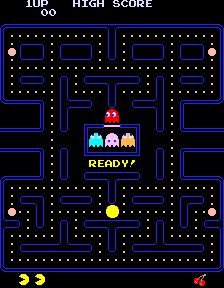
\includegraphics[width=0.31\textwidth]{pac-man-game1.png} &
    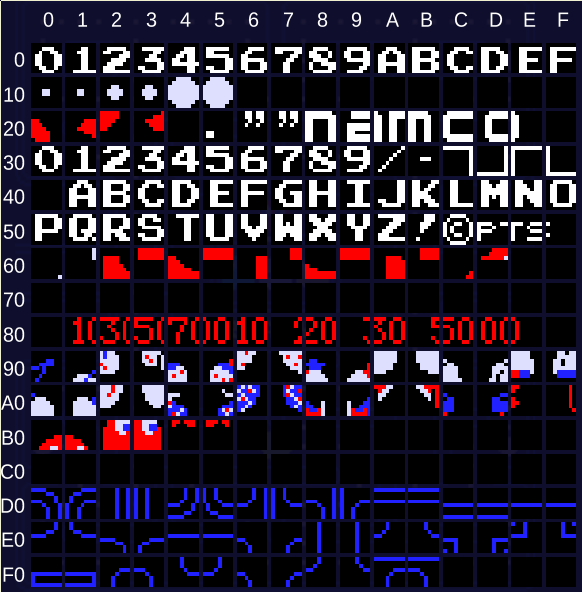
\includegraphics[width=0.31\textwidth]{pac-man-tiles.png} &
    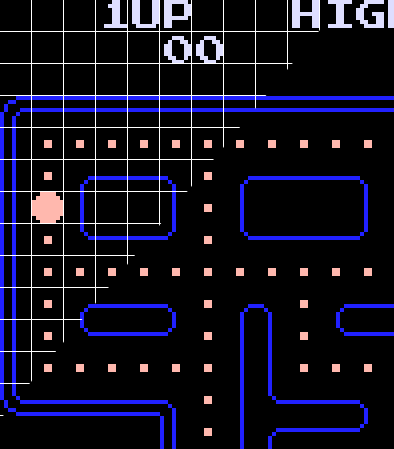
\includegraphics[width=0.31\textwidth]{pac-man-game-tiles1.png} \\
    (a) & (b) & (c)
  \end{tabular}
\caption{Pac-Man, Namco 1980. (a) Starting game screen,
  $224\times288$; (b) Tile set: 256 $8\times8$ tiles, 2 bpp; and (c) Game tile detail: $28\times36$ tiles, 2 bytes per tile (8b index, 5b palette)}
\label{fig:pacman}
\end{figure}

%% Program ROMS (16K total):
%% pacman.6e  0x0000 0x1000 4K
%% pacman.6f  0x1000 0x1000 4K
%% pacman.6h  0x2000 0x1000 4K
%% pacman.6j  0x3000 0x1000 4K
%%
%% Graphic ROMS (8K total):
%% pacman.5e  0x0000 0x1000 4K  "Maze and dots"  (256 * 16)
%% pacman.5f  0x1000 0x1000 4K  "Pac-man and ghosts" (256 * 16)
%%
%% PROMs
%% 82s123.7f  0x0000 0x0020 Color PROM (4 - 8 bpp)
%% 82s126.4a  0x0020 0x0100 "Color lookup" (256 X 4 bit); topmost bit likely not used
%%
%% Sound PROMs
%% 82s126.1m  0x0000 0x0100
%% 82s126.3m  0x0100 0x0100
%%
%% Good circuit details:
%% Pac-Man_MsPac-Man_Troubleshooting_Logic_Board_Part_2.pdf

\clearpage

\section{Framebuffers and Tiles}

Modern computers generally display raster images from frame buffers,
which provides individual control over the color of each possible
on-screen pixel.  This provides flexibility at the cost of memory
consumption.  For example, modern displays often represent colors with
24-bit \textsc{rgb} values, which for a $640\times480$ \textsc{vga}
display, requires
%
\[
640 \times 480 \times 3\ \text{bytes} = 921,600\ \text{bytes} = 900 \text{K}.
\]

This was a substantial amount of memory when \textsc{vga} was
introduced in 1987, so systems often reduced these demands by reducing
the number of bits per pixel and employing a \emph{palette}: a small,
very fast memory that translated color codes to color values.  For
example, a framebuffer might use~8 bits per pixel (bpp) to represent a
color index, allowing it to display~256 different colors at a time,
but would use a $256 \times 24$ palette memory that allowed each of
the~256 colors to be selected from a 24-bit color gamut.  This would
reduce framebuffer memory to
%
\[
640 \times 480 \times 1\ \text{bytes} = 307,200\ \text{bytes} =
300~\text{K}
\]
%
plus $256 \times 3 = 768$ bytes for the palette.  The aging
\textsc{gif} file format only supports indexed color, which can lead
to artifacts.

At the extreme, a~1~bpp (monochrome) framebuffer still consumes
%
\[
640 \times 480 = 307,000~\text{bits} = 38,400~\text{bytes} = 37.5~\text{K}.
\]

Tiles are effectively the palette approach applied also to sub-images.
A text-mode display (i.e., that can only display letters and numbers)
illustrates the idea: software is only able to control the identity of each character on the screen rather than each pixel.  Consider an $80\times
30$ character grid in which each character is taken from a font
of~256.  Each character is then $640 \div 80 = 8$ pixels wide and $480
\div 30 = 16$ pixels high (e.g., \figref{8x16-font}).  The character
grid requires
%
\[
80 \times 30 = 2,400~\text{bytes} = 2.34~\text{K},
\]
%
and the font, if it is only black-and-white, requires
%
\[
256 \times 1~\text{byte} \times 16~\text{rows} = 4096~\text{bytes} = 4~\text{K},
\]
%
which is a substantial reduction over the~37~K requirement for a
monochrome framebuffer with the same resolution.

The original \textsc{vga} text mode actually used~16 bits per
character:~8 to select one of~256 different glyphs, four to select the
background color, three for the foreground color, and one bit to make
the character blink.

\begin{figure}
  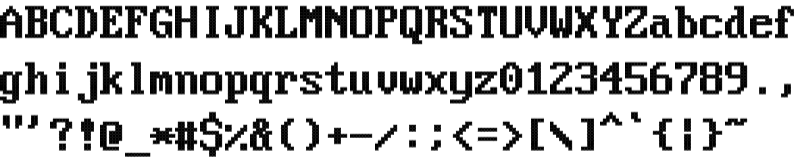
\includegraphics[width=\textwidth]{8x16-font.png}
  \caption{An $8 \times 16$ pixel font similar to that used on
    \textsc{ibm} \textsc{pc}s in the \textsc{vga} era.  Source:
  \url{https://fontstruct.com/fontstructions/show/1481905/dos-vga-9x16-1}}
  \label{fig:8x16-font}
\end{figure}

\clearpage

\begin{figure}
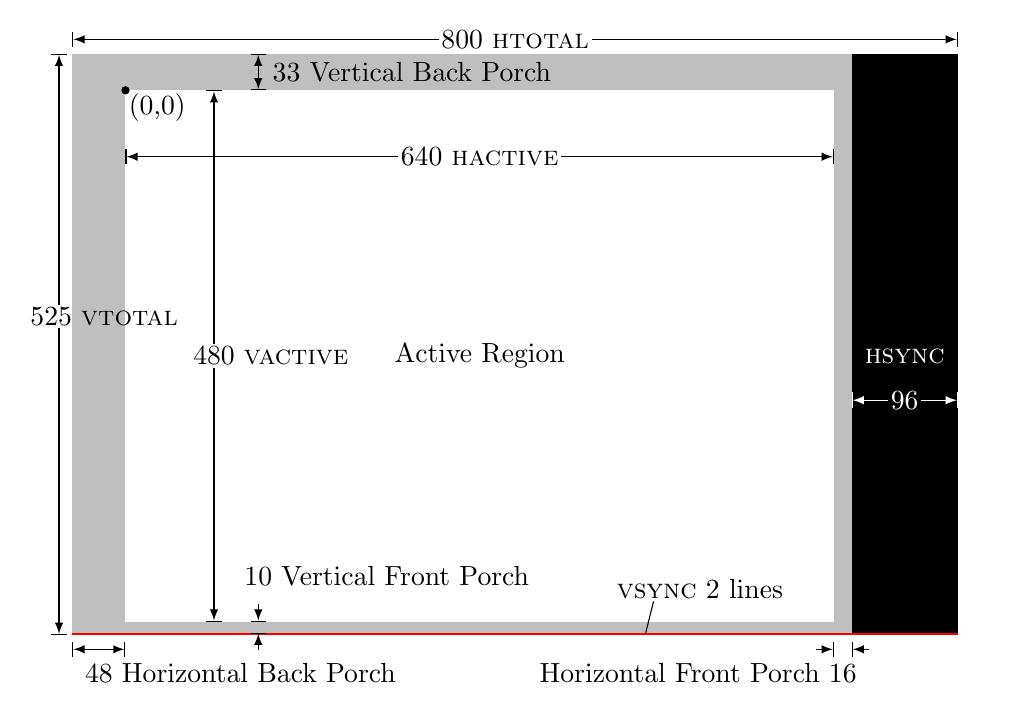
\begin{tikzpicture}[x=0.4pt,y=0.4pt,every node/.style={inner sep=1pt}]
  \fill [lightgray] (-48,33) rectangle ++(800,-525);
  \fill [white] (0,0) rectangle ++(640,-480);
  \fill [black] ($(640+16,33)$) rectangle ++(96,-525);
  \fill [red] ($(-48,-480-10)$) rectangle ++(800,-2);

  \node [circle,fill=black,inner sep=0pt,minimum width=3pt,minimum height=3pt]
  (0,0) {};  
  \node [below right] at (0,0) {(0,0)};

  \node at (320,-240) {Active Region};

  \draw [|<->|] (-48,46) --
  node [fill=white] {800 \textsc{htotal}} ++(right:800);

  \draw [|<->|] (0,-60) --
  node [fill=white] {640 \textsc{hactive}} ++(right:640);

  \draw [|<->|] (-60,33) --
  node [fill=white,yshift=10] {\ \rlap{\hspace{-12pt}525 \textsc{vtotal}}} coordinate (lab) ++(down:525);

  \draw [|<->|] (80,0) --
  node [fill=white] {480\rlap{ \textsc{vactive}}} ++(down:480);

  \draw [|<->|] (-48,-505) -- ++(48,0);
  \node [below] at (-24,-515) {48\rlap{ Horizontal Back Porch}};

  \draw [|<-] (640,-505) coordinate (here) -- ++(left:16);
  \draw [|<-]  (here) ++(16,0) -- ++(right:16);
  \node [below] at (648,-515) {\llap{Horizontal Front Porch }16}; % H front porch

  \node [white,fill=black] at ($(640 + 16 + 48,-240)$) {\textsc{hsync}};
  \draw [white,|<->|] (656,-280) -- node [fill=black] {96} ++(right:96);

  \draw [|<->|] ($(120,0)$) --
    node [right,xshift=4pt] {33 Vertical Back Porch} ++(up:33);

  \draw [|<-] ($(120,-480)$) -- ++(up:16);
  \draw [|<-] ($(120,-480-10)$) -- ++(down:16);
  \node [above] at ($(120,-480+30)$) {10\rlap{ Vertical Front Porch}}; % v front porch

  \node at ($(480,-450)$) (vslab) {\textsc{vsync}\rlap{ 2 lines}};
  \draw (vslab) -- (470,-490);

  \expandtotextwidth

\end{tikzpicture}  
  \caption{\textsc{vga} signal timing.  Horizontal dimensions are in
    pixels (25.175~MHz); vertical dimensions are in lines (31.46875~kHz). \\ Data from \url{http://www.tinyvga.com/vga-timing/640x480@60Hz}}
  \label{fig:vga-timing}
\end{figure}
% From http://www.tinyvga.com/vga-timing/640x480@60Hz

\section{The Video Graphics Array (VGA) Standard}

Most video arcade games and consoles in the '70s and '80s produced
raster-scanned, non-interlaced (progressive scan) \textsc{ntsc}-like
video:~60 frames per second, 262 lines, but we will follow the
slightly more modern Video Graphics Array (\textsc{vga}) standard,
which \textsc{ibm} introduced with their \textsc{ps}/2 line of
personal computers in~1987 and remains available.

The basic \textsc{vga} resolution is $640\times480$ at 60~fps with a
$25.175$~MHz dot clock: its timing is like a progressivly scanned
version of interlaced \textsc{ntsc} color video.  Modern \textsc{lcd}
monitors display \textsc{vga} signals by adapting to a wide variety of
horizontal and vertical frequencies while digitizing the analog
\textsc{rgb} \textsc{vga} signal.

\figref{vga-timing} illustrates \textsc{vga} timing.  Each line
is~800~pixel periods wide, but only~640 of those are displayed; the
remaining time is devoted to porches (blank periods) and
synchronization.  A new frame is displayed once every~525 line
periods, but only~480 lines are displayed.  Ten lines after the last
active line is a two-line-long vertical synchronization pulse followed
by~33 lines of additional ``back porch'' before the first line of the
next frame.


\begin{figure}
  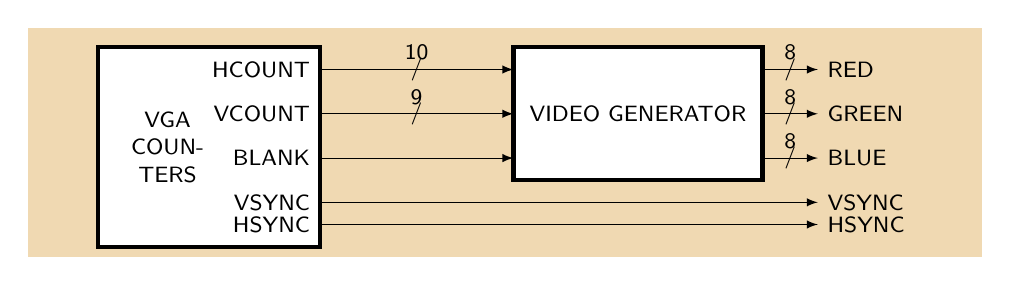
\begin{tikzpicture}[block diagram,y=8pt]
    \draw [block]  (-10,-5) rectangle node [text centered,text width=43pt,xshift=-15pt] {VGA COUNTERS} (-2,4);
    \draw [block] (5,-2) rectangle node {VIDEO GENERATOR} (14,4);
    \draw [->] (-2,3) node [left] {HCOUNT} \buswidth{10} ++(right:7);
    \draw [->] (-2,1) node [left] {VCOUNT} \buswidth{9} ++(right:7);
    \draw [->] (-2,-1) node[left] {BLANK}  -- ++(right:7);
    \draw [->] (14,3) \buswidth{8} ++(right:2) node [right] {RED};
    \draw [->] (14,1) \buswidth{8} ++(right:2) node [right] {GREEN};
    \draw [->] (14,-1) \buswidth{8} ++(right:2) node [right] {BLUE};

    \draw [->] (-2,-4) node [left] {HSYNC} -- ++(right:18)
      node [right] {HSYNC};
    \draw [->] (-2,-3) node [left] {VSYNC} -- ++(right:18)
      node [right] {VSYNC};

    \expandtotextwidth
    
  \end{tikzpicture}
  \caption{An abstract model of any \textsc{vga} video generator, such
    as one for tiles.  Counters generate horizontal and vertical
    coordinates as well as blanking and synchronization signals. The
    video generator translates these into three color signals.}
  \label{fig:video-logic}
\end{figure}

\section{VGA Counter Hardware}

\figref{video-logic} illustrates the structure of a \textsc{vga} video
generator: counters generate horizontal and vertical coordinate values
along with blanking signals, which are fed to a block that determines
the color of the pixel at those coordinates.

\figref{vga-counters} shows System Verilog that generates the
horizontal and vertical synchronization signals along with blanking
(true only during the active region) and horizontal and vertical
coordinates.

The logic for the horizontal synchronization signal is subtle to save
logic.  Horizontal synchronization occurs from count~$640 + 16 = 656$
through~count~$640 + 16 + 96 - 1 = 751$, which, in binary, are
%
\begin{verbatim}
10 1001 0000
10 1110 1111
\end{verbatim}
%
That is, \emph{hcount}[9:7] is 101 and \emph{hcount}[6:4] is not
000 or 111.  The logic for the blanking signal employs similar trickery.

I wrote a simple Verilator testbench for this code, which applies
a~25~MHz clock and reset and writes the simulation results as a
\emph{.vcd} file, which are displayed graphically in
\figref{vga-waveforms}.  These verify certain important behaviors.

\begin{figure}
\lstinputlisting{vga_counters.sv}
\caption{\emph{vga\_counters.sv}: Video counter module for \textsc{vga} in
  System Verilog}
\label{fig:vga-counters}
\end{figure}

\newcommand{\itempad}{\vspace{1.75\baselineskip}}

\begin{figure}

  \centering
  
  \includegraphics[width=0.95\textwidth]{vga_counters-reset.pdf}

  (a) Leaving reset; starting next frame after line 524; start of line 0

  \itempad
 
  \includegraphics[width=0.95\textwidth]{vga_counters-endl0.pdf}

  (b) End of Line 0 active: blanking then horizontal sync

  \itempad
  
  \includegraphics[width=0.95\textwidth]{vga_counters-endhs.pdf}

  (c) End of horizontal sync on line 0

  \itempad
  
  \includegraphics[width=0.95\textwidth]{vga_counters-start1.pdf}

  (d) Start of line 1; blanking ends
  
  \itempad

  \includegraphics[width=0.95\textwidth]{vga_counters-endactive.pdf}

  (e) End of active region; vertical sync

  \caption{Waveforms of the \textsc{vga} counters.\\ After a script \url{https://github.com/phillbush/vcd2svg} }
  \label{fig:vga-waveforms}

\end{figure}

\clearpage

\section{Framebuffer Design}

\figref{framebuffer} shows a design for a framebuffer: an address
generator fetching data from frame buffer memory.  Each word in the
memory contains the color code for a single pixel, here,~24 bits.  The
address of each pixel is $\textsc{hcount} + \textsc{vcount} \times
640$.  Multiplying by~640 is fairly easy since $640 = 512 + 128$, so
this could be implemented by adding \textsc{hcount}, \textsc{vcount}
shifted left~7 bits, and \textsc{vcount} shifted left~9 bits.

\begin{figure}
  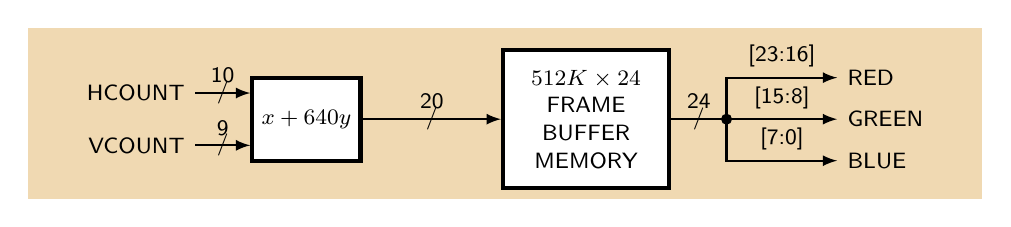
\begin{tikzpicture}[block diagram]
    \node [block,minimum height=30pt] (adr) {$x + 640 y$};
    \draw [<-,bus] ($(adr.north west)!0.2!(adr.south west)$) \buswidth{10} ++(left:2)
       node [left] {HCOUNT};
    \draw [<-,bus] ($(adr.north west)!0.8!(adr.south west)$) \buswidth{9} ++(left:2) node [left] {VCOUNT};
    \draw [->,bus] (adr.east) \buswidth{20} ++(right:5) coordinate (here);
    \node [block,minimum width=60pt, minimum height=50pt,
           text width=45pt,text centered,anchor=west] at (here) (mem)
          {$512\text{K} \times 24$ FRAME BUFFER MEMORY};
    \draw [->,bus] (mem.east) \buswidth{24} ++(right:2) \solder |- node [above,pos=0.75] {[23:16]}
             ++(4,1.5) node [right] {RED};
    \draw [->,bus] (mem.east) -- ++(right:2) |- node [above,pos=0.75] {[15:8]}
             ++(4,0) node [right] {GREEN};
    \draw [->,bus] (mem.east) -- ++(right:2) |- node [above,pos=0.75] {[7:0]}
    ++(4,-1.5) node [right] {BLUE};

    \expandtotextwidth
          
  \end{tikzpicture}
  \caption{A 24~bpp \textsc{vga} framebuffer built around a 1.5~MB memory}
  \label{fig:framebuffer}
\end{figure}

Indexed color using, say,~8~bpp, uses a smaller, 8-bit-wide
framebuffer memory then feeds the 8-bit color code to a $256 \times
24$ palette memory, which ultimately produces a 24-bit color.
\figref{indexed-fb} illustrates the structure of an indexed-color
framebuffer, which has traded some control over pixel colors for a
substantial reduction in memory.  Note that the overall function being
computed remains the same: the coordinate of each pixel in a
$640\times480$ grid is being mapped to a~24-bit color.

\begin{figure}
  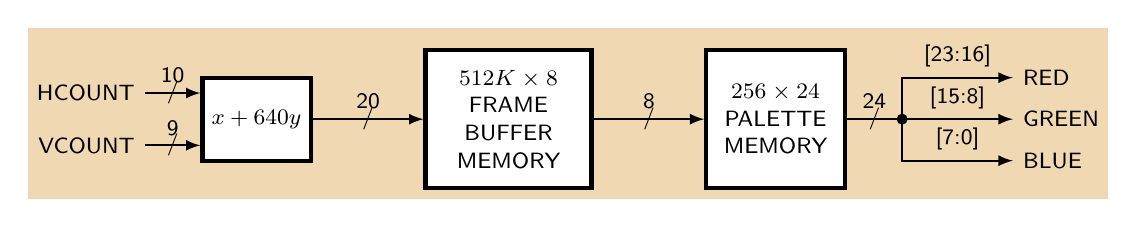
\begin{tikzpicture}[block diagram]

    \node [block,minimum height=30pt] (adr) {$x + 640 y$};
    \draw [<-,bus] ($(adr.north west)!0.2!(adr.south west)$)
    \buswidth{10} ++(left:2) node [left] {HCOUNT};
    
    \draw [<-,bus] ($(adr.north west)!0.8!(adr.south west)$)
    \buswidth{9} ++(left:2) node [left] {VCOUNT};
       
    \draw [->,bus] (adr.east) \buswidth{20} ++(right:4) coordinate (here);
    
    \node [block,minimum width=60pt, minimum height=50pt,
           text width=45pt,text centered,anchor=west] at (here) (mem)
          {$512\text{K} \times 8$ FRAME BUFFER MEMORY};

    \draw [->,bus] (mem.east) \buswidth{8} ++(right:4) coordinate (here);

    \node [block,minimum width=50pt, minimum height=50pt,
           text width=40pt,anchor=west,text centered] at (here) (pal)
          {$256 \times 24$ PALETTE MEMORY};
         
    \draw [->,bus] (pal.east) \buswidth{24} ++(right:2) \solder |- node [above,pos=0.75] {[23:16]}
             ++(4,1.5) node [right] {RED};
    \draw [->,bus] (pal.east) -- ++(right:2) |- node [above,pos=0.75] {[15:8]}
             ++(4,0) node [right] {GREEN};
    \draw [->,bus] (pal.east) -- ++(right:2) |- node [above,pos=0.75] {[7:0]}
    ++(4,-1.5) node [right] {BLUE};

    \expandtotextwidth
          
  \end{tikzpicture}
  \caption{An 8~bpp \textsc{vga} framebuffer that uses indexed colors
    from a palette memory.  Chaining a second memory to the first
    reduces memory consumption by nearly 2/3 without reducing the
    resolution or number of available colors.}
  \label{fig:indexed-fb}
\end{figure}

\clearpage

\begin{figure}

\begin{tikzpicture}[x=2pt,y=2pt]

  \node [anchor=north west,inner sep=0pt] at (0,0) {
\includegraphics[width=84pt]{pac-man-detail.png}};

  \draw [thin,white,step=8] (0,0) grid (42,-34);

  \node [below] at (20,-35) {(a) Image};

  \begin{scope}[shift={(60,0)}]

    \draw [step=8] (0,0) grid ++(42,-34);

    \foreach \x in {0,...,4} {
      \node [above] at ($(4+8*\x,0)$) {\footnotesize \x};
    }

    \foreach \y in {0,...,3} {
      \node [left] at ($(0,-4-8*\y)$) {\footnotesize \y};
    }

    \matrix [matrix of nodes,
      anchor=north west,
      nodes={minimum height=16pt,minimum width=16pt,inner sep=0pt,
        font={\footnotesize\ttfamily}}] at (-4pt,4pt) {
      D1 & DA & DA & DA & DA \\
      D3 & 10 & 10 & 10 & 10 \\
      D3 & 10 & E7 & DE & DE \\
      D3 & 14 & E9 & FC & FC \\
    };

    \node [above] at (20,6) {$c$};
    \node [left] at (-4,-16) {$r$};

    \node [below] at (20,-35) {(b) Tile Map};

  \end{scope}

  \begin{scope}[shift={(8,-45)}]

    \node [anchor=north west,inner sep=0pt] at (0,0) {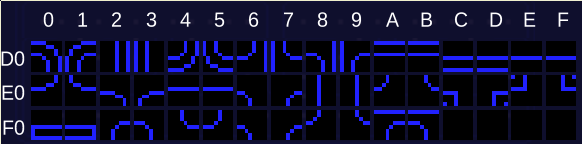
\includegraphics[width=180pt]{pac-man-tiles-2.png}};

    \node [below] at (50,-23) {(c) Tile Set (excerpt)};

  \end{scope}
  
  \begin{scope}[shift={(120,0)},scale=6]

    \draw [very thin,step=1,gray] (0,0) grid (10.5,-10.5);

    \draw [thick,step=8] (0,0) grid ++(10.5,-10.5);

    \foreach \x in {0,...,9} {
      \node [above] at ($(0.5+\x,0)$) {\footnotesize \x};
    }

    \foreach \y in {0,...,9} {
      \node [left] at ($(0,-0.5-\y)$) {\footnotesize \y};
    }
    
    \node [above] at (5,1) {$x$};
    \node [left] at (-1,-5) {$y$};

    \node [below right,inner sep=2pt,fill=white,text width=53pt,text badly ragged] at (2.3,-2.3) {Tile pixel coordinates $(i,j)$};

    \draw (2.3,-2.3) -- (1.5,-0.8);


    \node at (0.5,-0.5) {\tiny (0,0)};
    \node at (1.5,-0.5) {\tiny (1,0)};
    \node at (0.5,-1.5) {\tiny (0,1)};
    \node at (0.5,-7.5) {\tiny (0,7)};
    \node at (0.5,-8.5) {\tiny (0,0)};
    \node at (0.5,-9.5) {\tiny (0,1)};
    \node at (7.5,-0.5) {\tiny (7,0)};
    \node at (8.5,-0.5) {\tiny (0,0)};
    \node at (9.5,-0.5) {\tiny (1,0)};
    \node at (7.5,-7.5) {\tiny (7,7)};
    \node at (8.5,-7.5) {\tiny (0,7)};
    \node at (7.5,-8.5) {\tiny (7,0)};
    \node at (8.5,-8.5) {\tiny (0,0)};
    \node at (9.5,-8.5) {\tiny (1,0)};
    \node at (8.5,-9.5) {\tiny (0,1)};

    \node [below] at (4,-11) {(d) Pixel Coordinates};
    
  \end{scope}
  
  
\end{tikzpicture}

\caption{Tiles in Pac-Man: (a) Maze detail (b) Tile map: code for
  each tile (c) Partial tile set (d) Pixel and tile pixel coordinates}
  \label{fig:pac-man-detail}
\end{figure}

\begin{figure}
  \begin{tikzpicture}[block diagram]

    \node [block,text width=34pt,text centered,anchor=north west]
    (tma) {TILEMAP ADDRESS};
    

    \node [block,text width=32pt,text centered, anchor=west]
    at ($(tma.east) + (right:2)$) (tilemap)
    {$8192 \times 8$ TILEMAP RAM};

    \draw [->,bus] (tma.east) \buswidth{13} (tilemap.west);

    \node [block,text width=34pt,text centered,anchor=west] (tadr)
    at ($(tilemap.east) + (right:2)$) (tsa)
    {TILESET ADDRESS};

    \draw [->,bus] (tilemap.east) \buswidth{8} (tsa.west);

    \node [block,text width=30pt,text centered, anchor=west]
    at ($(tsa.east) + (right:2)$) (tileset)
    {$16 \text{K} \times 4$ TILESET RAM};

    \draw [->,bus] (tsa.east) \buswidth{14} (tileset.west);

    \node [block,text width=31pt,text centered, anchor=west]
    at ($(tileset.east) + (right:2)$) (palette)
    {$16 \times 24$ PALETTE RAM};

    \draw [->,bus] (tileset.east) \buswidth{4} (palette.west);

    \draw [->,bus] (palette.east) \buswidth{24} ++(right:2) node [right] {RGB};

    \node [anchor=east] at (-0.5,3) (hcount) {HCOUNT};
    \node [anchor=east] at (-0.5,1.5) (vcount) {VCOUNT};

    \draw [->,bus] (hcount.east) \buswidth{10} ++(right:1.5) -- ++(right:2) \solder \vlineto(tma.north);
    \draw [->,bus] (solder) -- ++(right:9) \buswidth{3} ++(right:2) -| ($(tsa.north) + (right:1)$);

    \draw [->,bus] (vcount.east) \buswidth{9} ++(right:1.5) \solder \vlineto(tma.north);
    \draw [->,bus] (solder) -- ++(right:11) \buswidth{3} ++(right:1) -| ($(tsa.north) + (left:1)$);

    \expandtotextwidth
          
  \end{tikzpicture}
  \caption{An $8\times8$ tile \textsc{vga} generator.  \textsc{hcount}
    and \textsc{vcount} deliver current pixel coordinates $(x,y)$.
    \textsc{tilemap address} transforms these to tile coordinates
    $(c,r)$ to compute to address in \textsc{tilemap ram} for the tile
    number $t$. \textsc{tileset address} combines $t$ with local tile
    coordinates $(i,j)$ to form the address for the pixel in
    \textsc{tileset ram}, which returns a 4-bit color code $c'$ that
    the \textsc{palette ram} translates to a 24-bit \textsc{rgb}
    value.}
  \label{fig:8x8-tiles}
\end{figure}

\section{Tile Generator Design}

A palette effectively compresses colors by expressing them using a
small number of codes; tiles take this one step further: a \emph{tile
map} memory holds a two-dimensional array of tile codes, one for each
tile on the screen; each code is used to index into memory that holds
the pixel color codes in the \emph{tile set}, a three-dimensional
array.  Finally, the color code is fed to a palette memory to look up
the final color. \figref{8x8-tiles} shows a block diagram of a tile
video generator.

\figref{pac-man-detail} illustrates the relationships among the tile
set, tile map, tile numbers, and pixels in an $8\times8$ tile system
like that in Pac-Man.  \figref{pac-man-detail}(a) shows a fragment of
the maze in the top left corner of the screen; each square is an
$8\times8$ pixel tile.  \figref{pac-man-detail}(b) is the top left
fragment of the tile map: the 2D array holding the code selecting each
on-screen tile.  Codes and the tiles they represent are shown in
\figref{pac-man-detail}(c).  \figref{pac-man-detail}(d) shows the
relationship between pixel coordinates and tile coordinates.  The tile
in row~0, column~0 starts at pixel $(0,0)$ and extends to pixel
$(7,7)$.  The tile to the right of this, at row~0, column~1, starts at
pixel $(8,0)$, which is tile pixel $(0,0)$.

\begin{figure}
\[
\begin{array}{rcll}
  (w,h) & & & \text{Tile width and height (pixels)} \\
  (x,y) & & & \text{Screen pixel coordinates} \\
  (c,r) & = & (\lfloor x \div w \rfloor, \lfloor y \div h \rfloor ) &
  \text{Tile column and row (tiles)} \\
  t & = & \text{tilemap}[c,r] &
  \text{Tile number (from tile map)} \\
  (i,j) & = & (x \bmod w, y \bmod h) &
  \text{Tile local coordinates (pixels)} \\
  c' & = & \text{tileset}[i,j,t] &
  \text{Pixel color code (from tile set)} \\
  (r,g,b) & = & \text{palette}[c'] &
  \text{Pixel color (from palette)} \\
\end{array}
\]
\caption{Calculating the color $(r,g,b)$ of the pixel at coordinates
  $(x,y)$ in an array of $w \times h$-pixel tiles.
  $\text{tilemap}[c,r]$ is the tile number at column $c$ and row $r$;
  $\text{tileset}[t,i,j]$ is the color code for pixel $(i,j)$ in tile
  $t$; and $\text{palette}[c']$ is the \textsc{rgb} color for color
  code $c'$.}
\label{fig:summary}
\end{figure}

\figref{summary} lists the rules for determining the pixel at screen
coordinates $(x,y$) in a regular array of $w \times h$-pixel tiles.  The
column and row $(c,r)$ of the tile containing the pixel is simply the
quotients from dividing each coordinate by the size of the tile.
These are used to look up the tile number in the tilemap array.  The
coordinates of the pixel within that tile (i.e., relative to the
tile's top left corner) $(i,j)$ is the remainder of these divisions.
These coordinates and the tile number are used to look up the color
code of the pixel in the tile set.  Finally, the color code is used to
look up the actual \textsc{rgb} color of the pixel.

Implementing a tile generator in hardware amounts to implementing the
rules in \figref{summary}.  First, we will choose fixed-size
$8\times8$ tiles: $(w,h) = (8,8)$.  Choosing these numbers to be fixed
powers of two greatly simplifies the implemention of the division
operations as well as the address calculations for the tile map and
tile set memories.  Square tiles are also natural for designing
graphics, although they are a little awkward for Roman letters.

Next, we need to determine the exact number of bits for data and
memory in \figref{summary}.  For \textsc{vga}, $x$ ranges from $0$ to
$639$, which we will represent as a 10-bit binary number whose bits we
will write $x_9\,x_8\cdots x_0$ (little-endian subscripts).
Similarly, $y$ ranges from $0$ to $479$, which takes~9 bits
$y_8\,y_7\cdots y_0$.  Note that these are active screen coordinates;
\textsc{vcount} actually uses~10 bits because it needs to count to~524.

Because $640 \div 8 = 80$ and $480 \div 8 =
60$, $c$ we need~7 bits for $c$: $c_6\,c_5\cdots c_0$, and 6~bits for
$r$: $r_5\,r_4\cdots r_0$.  Furthermore, the tile local coordinates
$(i,j)$ will each be~3 bits since each range over 0--7.

Thanks to our choice of 8-pixel-square tiles, dividing by the tile
size amounts to shifting right by~3 bits.  Calculating the tile column
and row $(c,r)$ along with the tile-local pixel coordinates $(i,j)$
amounts to splitting each pixel coordinate into a~3-bit local tile
coordinate and a~7- or 6-bit tile column and row:
%
\begin{equation}
(\underbrace{x_9\,x_8\cdots x_3}_{c_6\,c_5\cdots c_0}\,
\underbrace{x_2\,x_1\,x_0}_{i_2\,i_1i_0}
,\ \underbrace{y_8\,y_7\cdots y_3}_{r_5\,r_4\cdots r_0}\,
\underbrace{y_2\,y_1\,y_0}_{j_2\,j_1\,j_0}).
\label{eq:column-row}
\end{equation}

The tile map needs to hold an $80 \times 60$ array, so its entries
could be addressed as $c + 80r$, but this requires a constant
multiplication and addition.  While this could be done with three
additions because $80 = 64 + 16$, it is easier to round $80$ up to the
next power of two: $128$.  This wastes some memory ($128 \times 64 =
8192$ versus $80 \times 60 = 4800$), but this memory is a small
fraction of the total available on the \textsc{fpga}, which contains
minimum-sized memory chunks, anyway.  Also,~4800 is greater than~4096,
which was the previous natural power-of-two size for the memory.

To support~256 tiles with a $128 \times 64$ tile map, the tile number
$t$ will be~8 bits, the address to tile map memory will be~13 bits
($128 \times 64 = 8192 = 2^{13}$), and the address for the tile map
memory will consist of the~6 $r$ bits for the \textsc{msb}s followed
by the~7 $c$ bits:
%
\begin{equation}
t_7\,t_6\cdots t_0 = \text{tilemap}[r_5\,r_4\cdots r_0\,c_6\,c_5\cdots c_0].
\label{eq:tilemap}
\end{equation}
%
Putting the column number in the least significant bits gives a
row-major layout: tiles in a row appear in successive memory
locations; tiles in the row below appear in memory after all the tiles
for the row above.

Pac-Man used 4-bit color codes; to store the color codes
for~256~$8\times8$ tiles takes a~4-bit-wide memory with $256 \times 8
\times 8 = 16384 = 2^{14}$ entries.  Again, addressing this memory is
easy because the tiles are a power of two: the least significant bits
of the~15-bit address starts with~3 bits of $i$ (the horizontal
tile-local coordinate) followed by~3 bits of $j$ (the vertical
tile-local coordinate) followed by the~8 bit tile number.
%
\begin{equation}
c'_3\,c'_2\,c'_1\,c'_0 = \text{tileset}[t_7\,t_6\cdots t_0\,j_2\,j_1\,j_0\,i_2\,i_1\,i_0].
\label{eq:tileset}
\end{equation}
%
This is also a row-major layout: the pixels for a tile appear as eight
rows of pixels; data for each tile starts at a multiple of~64 pixels.

\clearpage

\newcommand{\datasize}{\fontsize{7}{6}\selectfont}

\begin{figure}
  \begin{minipage}[b]{0.3\textwidth}
    \centerline{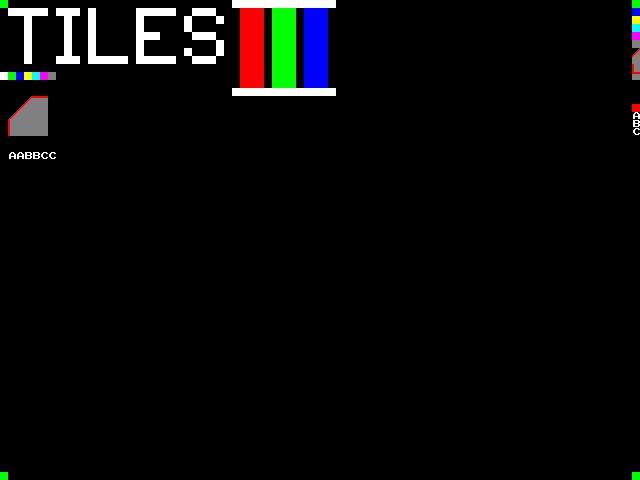
\includegraphics[width=1\textwidth]{tiles1.png}}
    
    \centerline{(a) Image}
  \end{minipage}\hfill
  \begin{minipage}[b]{0.29\textwidth}   
{\datasize\begin{verbatim}
02 00 00 00 00 00 00 00 00 00 ... 00
00 01 01 01 01 01 00 01 01 01 ... 00
00 00 00 01 00 00 00 00 01 00 ... 00
00 00 00 01 00 00 00 00 01 00 ... 00
00 00 00 01 00 00 00 00 01 00 ... 00
00 00 00 01 00 00 00 00 01 00 ... 00
00 00 00 01 00 00 00 00 01 00 ... 00
00 00 00 01 00 00 00 01 01 01 ... 00
00 00 00 00 00 00 00 00 00 00 ... 00
...
\end{verbatim}}

  \vspace{-1\baselineskip}
  \centerline{(b) Tilemap}
  
  \end{minipage}\hfill
  \begin{minipage}[b]{0.22\textwidth}  
{\datasize
\begin{verbatim}
...
00 00 00 0f 0f 0f 00 00
00 00 0f 0f 00 0f 0f 00
00 0f 0f 00 00 00 0f 0f
00 0f 0f 00 00 00 0f 0f
00 0f 0f 0f 0f 0f 0f 0f
00 0f 0f 00 00 00 0f 0f
00 0f 0f 00 00 00 0f 0f
00 00 00 00 00 00 00 00

00 0f 0f 0f 0f 0f 0f 00
00 0f 0f 00 00 00 0f 0f
00 0f 0f 00 00 00 0f 0f
00 0f 0f 0f 0f 0f 0f 00
00 0f 0f 00 00 00 0f 0f
00 0f 0f 00 00 00 0f 0f
00 0f 0f 0f 0f 0f 0f 00
00 00 00 00 00 00 00 00
...
\end{verbatim}
}
  \vspace{-1.25\baselineskip}
\centerline{(c) Tileset}
  \end{minipage}\hfill
  \begin{minipage}[b]{0.1\textwidth}  
  {\datasize
\begin{verbatim}
00 00 00 00
FF 00 00 00
00 FF 00 00
00 00 FF 00
FF FF 00 00
00 FF FF 00
FF 00 FF 00
80 80 80 00
00 00 00 00
00 00 00 00
00 00 00 00
00 00 00 00
00 00 00 00
00 00 00 00
00 00 00 00
FF FF FF 00
\end{verbatim}
  }
  \vspace{-0.5\baselineskip}
  \centerline{(d) Palette}
  \end{minipage}

  \caption{(a) Image generated by \emph{tiles2ppm}.  (b) The Tilemap
    file: 02 is a green square; the 01s (white squares) spell out
    ``TI.''  (c) ``A'' and ``B'' tiles in the Tileset.  (d) The
    16-color palette (black, red, green, blue, yellow, etc.).  Each 24-bit value is padded to be 32-bit aligned.}
  \label{fig:tile-output}
\end{figure}

\begin{figure}
  \lstinputlisting[language=C,
    basicstyle=\fontsize{9}{9}\selectfont\ttfamily]{tiles2ppm.c}
  \caption{\emph{tiles2ppm.c}:
    An untimed C model of the tile video generator that loads
    tilemap, tileset, and palette binary files using
    \emph{mmap}() then calculates the color of each pixel
    and writes it as a \textsc{ppm} format file.}
\label{fig:tile-sw}
\end{figure}

\section{A Software Prototype for the Tile Generator}

Complex hardware is always designed by creating an increasingly
detailed series of models.  The first is very abstract (e.g., a
statement like ``let's display graphics with tiles''); the last is the
implementation itself.  At each step, earlier models guide the
implemention of the next, details are added, and each model is checked
for conformance with the last.  \figref{8x8-tiles} is one such model
of our tile generator; it will guide our eventual System Verilog model
that we will use to implement the circuit on an \textsc{fpga}.

Designers often use an executable software model as part of the
development process.  It can be very abstract and only model the
algorithm, it can be a very detailed ``cycle-accurate'' model that
models clock-by-clock hardware behavior, or something in between.

\figref{tile-sw} shows an abstract software model coded in C designed
to verify the ``algorithm'': effectively \figref{8x8-tiles} and
equations \equref{column-row}, \equref{tilemap}, and \equref{tileset}.
It is also useful for testing binary palette, tileset, and tilemap
data, the filenames for which are supplied on the command line.  It
runs the algorithm to generate a $640\times480$ image and writes the
result as a \textsc{ppm}
file,\footnote{\url{https://netpbm.sourceforge.net/doc/ppm.html}} an
uncompressed image format suitable for previewing.  The body of the
nested \emph{for} loops in \emph{main}() implement the rules in
\figref{summary}; all the rest is testbench scaffolding.

\figref{tile-output} shows the output of this program for a test
tilemap, tileset, and palette.  With a text editor, I created text
files for each then converted them to binary using the \emph{xxd}
Linux command-line utility.  The tilemap file is~64 lines of~128 bytes
each; the tileset file is~256 tiles, each~8 lines of~8 bytes each (4
bits only); the palette file is~16 lines of four bytes each.

\section{Tile Hardware Pipeline Design}

From \figref{8x8-tiles}, the tile generator needs three small
memories: tilemap, tileset, and palette.  Each is a different size
(both word size and number of words), but similar in that they both
need to retrieve information for the video generator and we want to be
able to read and write to them from software.  Arbitrating memory
access between \textsc{cpu} and graphics controller has long been a
challenge, but our \textsc{fpga} provides a convenient solution: the
on-chip block \textsc{ram}s are dual-ported, meaning they can perform
two independent read or write operations every cycle, one in each
clock domain. We will dedicate one port to the video generator (which
will only read) and the other to the \textsc{cpu} (technically, an the
Avalon agent bus interface coming from the \textsc{hps}); each will
run on their own clock.

We will use the parametric two-port \textsc{bram} module in
\figref{twoportbram} for these three memories.  To instantiate it, you
supply two compile-time two parameters: \textsc{data\_bits} and
\textsc{address\_bits}.  The body is coded so that Quartus will
marshal the appropriate collection of M10K blocks to implement it.

\begin{figure}
  \lstinputlisting{twoportbram.sv}
  \caption{\emph{twoportbram.sv}: Parametric two-port synchronous
    \textsc{bram} module for implementing the tilemap, tileset, and
    palette memories.  The second port will enable software access to
    the memory.  Note that each port has its own clock.}
  \label{fig:twoportbram}
\end{figure}

\begin{figure}
  \begin{tikzpicture}[block diagram]
    
    \node [block,text width=45pt,text centered,minimum height=110pt] (cntrs)
          {VGA COUNTERS};

    \node [block,text width=34pt,text centered,anchor=north west]
    at ($(cntrs.north east) + (0.5,-4)$)
    (tma) {TILEMAP ADDRESS};
    
    \node [block,text width=32pt,text centered, anchor=west,inner ysep=7pt]
    at ($(tma.east) + (right:2)$) (tilemap)
    {$8192 \times 8$ TILEMAP RAM};
    \clockport (tilemap.south);

    \draw [->,bus] (tma.east) \buswidth{13} (tilemap.west);

    \node [block,text width=34pt,text centered,anchor=west] (tadr)
    at ($(tilemap.east) + (right:1.8)$) (tsa)
    {TILESET ADDRESS};

    \draw [->,bus] (tilemap.east) \buswidth{8} (tsa.west);

    \node [block,text width=30pt,text centered, anchor=west,inner ysep=7pt]
    at ($(tsa.east) + (right:1.8)$) (tileset)
    {$16 \text{K} \times 4$ TILESET RAM};
    \clockport (tileset.south);

    \draw [->,bus] (tsa.east) \buswidth{14} (tileset.west);

    \node [block,text width=31pt,text centered, anchor=west,inner ysep=7pt]
    at ($(tileset.east) + (right:1.8)$) (palette)
    {$16 \times 24$ PALETTE RAM};
    \clockport (palette.south);

    \draw [->,bus] (tileset.east) \buswidth{4} (palette.west);

    \draw [->,bus] (palette.east) \buswidth{24} ++(right:1.5) coordinate (rgb)
    node [right] {RGB};

    \node [anchor=east] at ($(cntrs.north east) + (down:0.7)$) (hcount) {HCOUNT};
    \node [anchor=east] at ($(cntrs.north east) + (down:2)$) (vcount) {VCOUNT};

    \node [anchor=east] at ($(cntrs.south east) + (up:2.8)$) (blank) {BLANK};
    \node [anchor=east] at ($(cntrs.south east) + (up:1.8)$) (hs) {HS};
    \node [anchor=east] at ($(cntrs.south east) + (up:0.8)$) (vs) {VS};

    \draw [->,bus] (hcount.east) \buswidth{10} ++(right:1.5)
    -- ++(right:11) \buswidth{3} ++(right:1) -| ($(tsa.north) + (right:0.75)$);
    \draw [<-,bus] ($(tma.north) + (right:0.75)$) \vlineto(hcount.east) \solder;

    \draw [->,bus] (vcount.east) \buswidth{9} ++(right:1.5)
    -- ++(right:10) \buswidth{3} ++(right:1) -| ($(tsa.north) + (left:0.75)$);
    \draw [<-,bus] ($(tma.north) + (left:0.75)$) \vlineto(vcount.east) \solder;
    
    \draw [->] (blank) \hlineto(rgb) coordinate (blankout) node [right] {BLANK};
    \draw [->] (hs) \hlineto(rgb) coordinate (hsout) node [right] {HS};
    \draw [->] (vs) \hlineto(rgb) node [right] {VS};

    \node [block,minimum height=15pt, minimum width=10pt]
    at ($(hcount)!(tilemap)!($(hcount) + (right:1)$)$) (pipe0) {};
    \clockport (pipe0.south);

    \node [block,minimum height=20pt, minimum width=10pt]
    at ($($(hs)!0.5!(blank)$)!(tilemap)!($(hsout)!0.5!(blankout)$)$)
    (pipe1) {};
    \clockport (pipe1.south);

    \node [block,minimum height=20pt, minimum width=10pt]
    at ($($(hs)!0.5!(blank)$)!(tileset)!($(hsout)!0.5!(blankout)$)$)
    (pipe2) {};
    \clockport (pipe2.south);

    \node [block,minimum height=20pt, minimum width=10pt]
    at ($($(hs)!0.5!(blank)$)!(palette)!($(hsout)!0.5!(blankout)$)$)
    (pipe3) {};
    \clockport (pipe3.south);

    \draw [<->,bus] ($(tilemap.north west) + (right:0.5)$) -- ++(up:4)
    node [above] {TM PORT 13/8};

    \draw [<->,bus] (tileset.north) -- ++(up:4)
    node [above] {TS PORT 14/4};

    \draw [<->,bus] (palette.north) -- ++(up:4)
    node [above,xshift=5pt] {PALETTE PORT 4/24};

    \expandtotextwidth
          
  \end{tikzpicture}
  \caption{A pipelined $8\times8$ tile \textsc{vga} generator with
    ports for accessing the tilemap, tileset, and palette memories and
    a \textsc{blank} signal needed by the \textsc{vga} \textsc{dac}.}
  \label{fig:tiles-pipelined}
\end{figure}

\begin{figure}
  \lstinputlisting[lastline=35]{tiles.sv}
  \caption{\emph{tiles.sv}: The tile video generator (part 1/2).  This
    interface takes in the \textsc{vga} pixel clock and generates
    the \textsc{vga} color and synchronization signals.  It also
    exposes read/write memory ports for the tilemap, tileset, and palette.}
  \label{fig:tiles-p1}
\end{figure}

\begin{figure}
  \lstinputlisting[firstline=37]{tiles.sv}
  \caption{\emph{tiles.sv}: The tile video generator (part 2/2).  This
    instatiates the \textsc{vga} counters and connects the three
    memories and pipeline register groups following
    \figref{tiles-pipelined}.  Note that the memory ports have their own clock.}
  \label{fig:tiles-p2}
\end{figure}

\figref{tiles-pipelined} shows a block diagram for the core of the
\textsc{vga} tile generator.  This is \figref{8x8-tiles} augmented
with the \textsc{vga} counters block, second memory ports for software
access to the three synchronous block \textsc{rams}, and pipeline
registers on the \textsc{hcount}, \textsc{blank}, and \textsc{hs}
signals.

The block diagram of \figref{8x8-tiles} only models function, not
timing; \figref{tiles-pipelined} models timing and adds pipeline
registers to remain consistent.  The block \textsc{ram}s on the
\textsc{fpga} are synchronous: a read operation always takes a cycle,
so the output of the tilemap memory comes a cycle after its address.
Because the \textsc{hcount} signal changes every pixel cycle, feeding
\textsc{hcount} directly to the tileset address generator would be
inconsistent (it would be one higher than it should be, causing a
graphical glitch), so I inserted a pipeline register on
\textsc{hcount} between the output of the \textsc{vga} counter and the
tileset address generator.  Similar concerns apply to the
\textsc{blank} and \text{hs} signals, which need to be generated in
alignment with the pixel color data.

It would be natural to add pipeline registers on \textsc{vcount}
and \textsc{vs}, but because \textsc{vcount} only changes at the end
of each scanline, we can just use its unpipelined value without any
change in behavior.  Omitting pipeline registers on the \textsc{vs}
signal does change its timing slightly, but the monitor ignores a~3
cycle (119~ns) delay on this~60~Hz signal.

\figref{tiles-p1} is the first half of code implementing the pipelined
tile generator in \figref{tiles-pipelined}.  It consists of the module
interface (clock and reset, \textsc{vga} signals, and three memory
ports), local wires and registers, and an instance of the \textsc{vga}
counter module from \figref{vga-counters}.

\figref{tiles-p2} is the second half of the tile generator hardware.
It instantiates the three memories and implements the three groups of
pipeline registers.  The first port of each memory is used for video
generation and operated in read-only mode.

The Tilemap address generator is just the expression \{
\emph{vcount}[8:3], \emph{hcount}[9:3] \} fed to the tilemap's
\emph{addr1}, which is too small to warrant a separate module.
Similarly, the Tileset address generator is the expression \{
\emph{tilenumber}, \emph{vcount}[2:0], \emph{hcount1} \}.

\begin{figure}[p]
  \begin{tikzpicture}[block diagram]

    \node [block,minimum width=230pt, minimum height=50pt]
    (pipeline) {};
    \node [yshift=-5pt] at (pipeline) {VGA TILE PIPELINE};

    \path ($(pipeline.north west) + (1.5,0)$)
    coordinate (tmp di) node [below] {DI:8}
    ++(right:2) coordinate(tmp we) node [below] {WE}
    +(0,-1) node [below] {TILEMAP}
    ++(right:2) coordinate(tmp a) node [below] {A:13}
    ++(-2,-5) coordinate(tmp do) node [above] {DO:8};
    
    \path ($(pipeline.north) + (-2,0)$)
    coordinate (tsp di) node [below] {DI:4}
    ++(right:2) coordinate(tsp we) node [below] {WE}
    +(0,-1) node [below] {TILESET}
    ++(right:2) coordinate (tsp a) node [below] {A:14}
    ++(-2,-5) coordinate (tsp do) node [above] {DO:4};

    \path ($(pipeline.north east) + (-5,0)$)
    coordinate (palette di) node [below] {DI:24}
    ++(right:2) coordinate(palette we) node [below] {WE}
    +(0,-1) node [below] {PALETTE}
    ++(right:2) coordinate(palette a) node [below] {A:4}
    ++(-2,-5) coordinate(palette do) node [above] {DO:24};

    \draw [<-] (tmp we) -- ++(up:1);
    \draw [<-] (tsp we) -- ++(up:1);
    \draw [<-] (palette we) -- ++(up:1);

    \node [block,minimum width=30, minimum height=10pt, anchor=south]
    at ($(palette di) + (0,1.5)$) (creg) {};
    \node [left] at (creg.west) {CREG};
    \draw ($(creg.south west)!0.33!(creg.south east)$) \vlineto (creg.north);
    \draw ($(creg.south west)!0.66!(creg.south east)$) \vlineto (creg.north);
    \draw [->,bus] (creg.south) \vlineto(palette di);

    \draw [bus,->] ($(pipeline.north west) + (-1,4)$) coordinate (writedata)
    node [left] {WRITEDATA} \buswidth{8} ++(right:1)
    -| (creg.north);
    \draw [bus,<-] (tmp di) \vlineto(writedata) \solder;
    \draw [bus,<-] (tsp di) \vlineto(writedata) \solder;

    \draw [bus,->] ($(writedata) + (0,1.5)$) coordinate (address)
    node [left] {ADDRESS} \buswidth{15} ++(right:1) -| (palette a);
    \draw [bus,<-] (tmp a) \vlineto(address) \solder;
    \draw [bus,<-] (tsp a) \vlineto(address) \solder;

    \draw [->] ($(writedata) + (0,-3)$) node [left] {WRITE} -- ++(right:1);
    \draw [->] ($(writedata) + (0,-1.5)$) node [left] {CHIPSELECT} -- ++(right:1);

    \draw [block] ($(palette do) + (1,-3)$) coordinate (cregm)
    -- ++(1,0.5) -- ++(0,1) -- ++(-1,0.5) -- cycle;
    \draw [bus] ($(cregm) + (0.5,0.25)$) -- ++(down:0.5);
    \draw [bus] ($(cregm) + (0,0.25)$) -| (palette do);
    \draw [bus] ($(cregm) + (0,1)$) \hlineto(palette do) \solder;
    \draw [bus] ($(cregm) + (0,1.75)$) \hlineto(palette do) \solder;

    \draw [block] ($(cregm) + (3,-2)$) coordinate (mux)
    -- ++(1,0.5) -- ++(0,1) -- ++(-1,0.5) -- cycle;
    \draw [bus] ($(mux) + (0.5,0.25)$) -- ++(down:0.5);
    \draw [bus] ($(cregm) + (1,1)$) -- ++(right:1) |- ($(mux) + (0,1.75)$);
    \draw [bus] (tsp do) |- ($(mux) + (0,1)$);
    \draw [bus] (tmp do) |- ($(mux) + (0,0.25)$);
    \draw [->,bus] ($(mux) + (1,1)$) \buswidth{8} ++(right:2)
    coordinate (readdata) node [right] {READDATA};

    \draw [->,bus] ($(pipeline.south east) + (up:4)$) \buswidth{24}
    ++(right:1) \hlineto(readdata) node [right] {RGB};

    \draw [->] ($(pipeline.south east) + (up:3)$) \hlineto(readdata)
    node [right] {BLANK};
        
    \draw [->] ($(pipeline.south east) + (up:2)$) \hlineto(readdata)
    node [right] {HS};

    \draw [->] ($(pipeline.south east) + (up:1)$) \hlineto(readdata)
    node [right] {VS};

  
    \expandtotextwidth
    
  \end{tikzpicture}
  \caption{The \textsc{vga} tile generator component with an Avalon MM
    Agent interface}
  \label{fig:tile-component}
\end{figure}


\begin{figure}[p]
\[  
\begin{array}{*3{c@{\,}}*3{@{\ \ }*4{c@{\,}}}@{\quad}l}
  a_{14}&a_{13}&a_{12}&a_{11}&a_{10}&a_{9}&a_{8}&a_{7}&a_{6}&a_{5}&a_{4}&a_{3}&a_{2}&a_{1}&a_{0}\\
  \hline
 0&0&m_{12}& m_{11}&m_{10}&m_9&m_8& m_7&m_6&m_5&m_4 &m_3&m_2&m_1&m_0 &\text{Tilemap} \\
 0&1&0& 0&0&0&0& 0&0&p_3&p_2 &p_1&p_0&b_1&b_0 &\text{Palette} \\
 1&s_{13}&s_{12}& s_{11}&s_{10}&s_9&s_8& s_7&s_6&s_5&s_4 &s_3&s_2&s_1&s_0 &\text{Tileset} \\
  \end{array}
\]

(a) Address Encoding:  the $a$ are
bus (byte) address bits; $m$ are Tilemap address bits; $p$ are Palette
(color number) bits, $b$ are ``byte'' bits, and the $s$ are Tileset
address bits.

\begin{center}
\begin{tabular}{cll}
  \textbf{Byte Offset} & \textbf{Region} & \textbf{Contents} \\
  \hline
  \texttt{0000 - 1FFF} & Tilemap & 8K, 8 bit tile numbers \\
  \texttt{2000 - 203F} & Palette & 64 bytes, 4 bytes per 24-bit color \\
  \texttt{4000 - 7FFF} & Tileset & 16K, 4 bit color numbers (LSBs) \\
  \hline
\end{tabular}

\medskip

(b) Memory Map
\end{center}

\begin{tabular}{r|c|c|c|c|}
\multicolumn{1}{c}{} &
  \multicolumn{1}{c}{0} &
  \multicolumn{1}{c}{1} &
  \multicolumn{1}{c}{2} &
  \multicolumn{1}{c}{3} \\
  \cline{2-5}
  0 & red 0 & green 0 & blue 0 & write 0 \\
  \cline{2-5}
  4 & red 1 & green 1 & blue 1 & write 1 \\
  \cline{2-5}
\multicolumn{1}{c}{} & \multicolumn{4}{c}{$\vdots$} \\
  \cline{2-5}
  60 & red 15 & green 15 & blue 15 & write 15 \\
  \cline{2-5}
\end{tabular}
\hfill
\begin{minipage}{0.45\textwidth}

  \footnotesize\parskip=0.15\baselineskip\raggedright

Reading from red $n$/green $n$/blue $n$ returns
the component from color $n$ in memory.

Writing to red $n$/green $n$/blue $n$ stores the component in
\emph{creg}; $n$ ignored.

Reading from write $n$ returns 0.

Writing to write $n$ writes \emph{creg} to color $n$; the written value is ignored.
\end{minipage}

\medskip

\centerline{(c) Bytes in the Palette region}

\caption{Software model of the tile component}
\label{fig:memmap} 
\end{figure}

\section{Implementing VGA Tiles: an Avalon MM Agent}

We want to control the tile generator from software, so we will create
a Platform Designer component for the tile generator that includes an
Avalon Memory-Mapped Agent port.  The basic challenge is adapting this
protocol to the three memory port interfaces in \figref{tiles-p2}.

\figref{tile-component} shows the datapath for the interface.  We will
choose an 8-bit wide bus interface because the tilemap memory is~8
bits wide and the tileset memory is~4 bits wide.  The 24-bit wide
palette memory is a little problematic, but this is easier to deal
with than adapting the software to work with a 32-bit interface.

The tilemap memory port is the easiest to connect: the address and
data-in bits can come straight from the bus.  When the software reads
from this memory, the mux in the lower right will route its data-out
bits to \emph{readdata} on the interface.

The tileset memory is almost as easy: the address bits can come
straight from the bus.  We only need~4 data bits, so we can take those
from the lowest~4 bus bits.  This may seem like a waste, but the extra
bits are never stored in the tileset memory.

The 24-bit-wide palette memory is more challenging.  While the
\textsc{bram}s have the ability to have different width ports, we will
solve it by allowing the software to write a byte at a time to a
single~24-bit register (\emph{creg} in \figref{tile-component}) that
can ultimately be written to the palette memory.  Reading palette
memory gives~3 bytes; another mux selects one of them.

\figref{memmap} shows the software model, which will dictate the
datapath control for \figref{tile-component}.

\figref{memmap}(a) shows the encoding of bus addresses.  We have three
memory regions: the 8K Tilemap; the 16K Tileset, and the 16-entry
Palette.  We start with the largest region (Tileset), which
requires~14 address bits, and add a leading~1 to distinguish it from
the other regions.  The Tilemap region only requires~13 address bits,
so we set its top two address bits to~00.  This leaves the code~01,
which will select the palette.  Because each color is~24 bits, we need
at least three byte addresses per color, but it is easier to use a
power of two, so we will use~4 bytes per color.  The two least
significant bits will indicate the color component (byte) and the next
four will select the color number (0--15).

\figref{memmap}(b) is a memory map, essentially the address encoding
in hexadecimal.

To make it possible to write palette colors into memory sequentially
one byte at a time, writing to the first three bytes of each four-byte
color only writes into one of the three bytes of the \emph{creg}
register, not to palette memory.  When the fourth byte is written
(addresses 3, 7, 11, \ldots), the~24-bit \emph{creg} is written to
palette memory at the byte address shifted right~2 bits.
\figref{memmap}(c) depicts the byte-by-byte layout of the palette
region.

\begin{figure}
  \lstinputlisting[firstline=40,
    basicstyle=\fontsize{9}{9}\selectfont\ttfamily]{vga_tiles.sv}
  \vspace{-\baselineskip}
  \caption{\emph{vga\_tiles.sv}: The tile generator component, which adds
    an Avalon MM Agent port to the video generation hardware}
  \label{fig:vga-tiles}
\end{figure}

\figref{vga-tiles} shows the System Verilog code for the tile
component in \figref{tiles-pipelined}.  The combinational block
performs address decoding by examining \emph{chipselect} and address
bits.  Avalon's single-cycle writes demands this be combinational: the
\textsc{bram} write enable signals must appear in the same cycle as
\emph{write}.  The multiplexers that steer data to the \emph{readdata}
port are implicit in the various assignments to
\emph{readdata}.  The sequential block implements creg; the bits of
\emph{creg\_write} select which byte is loaded from \emph{writedata}
on a write to palette addresses.

\begin{figure}
  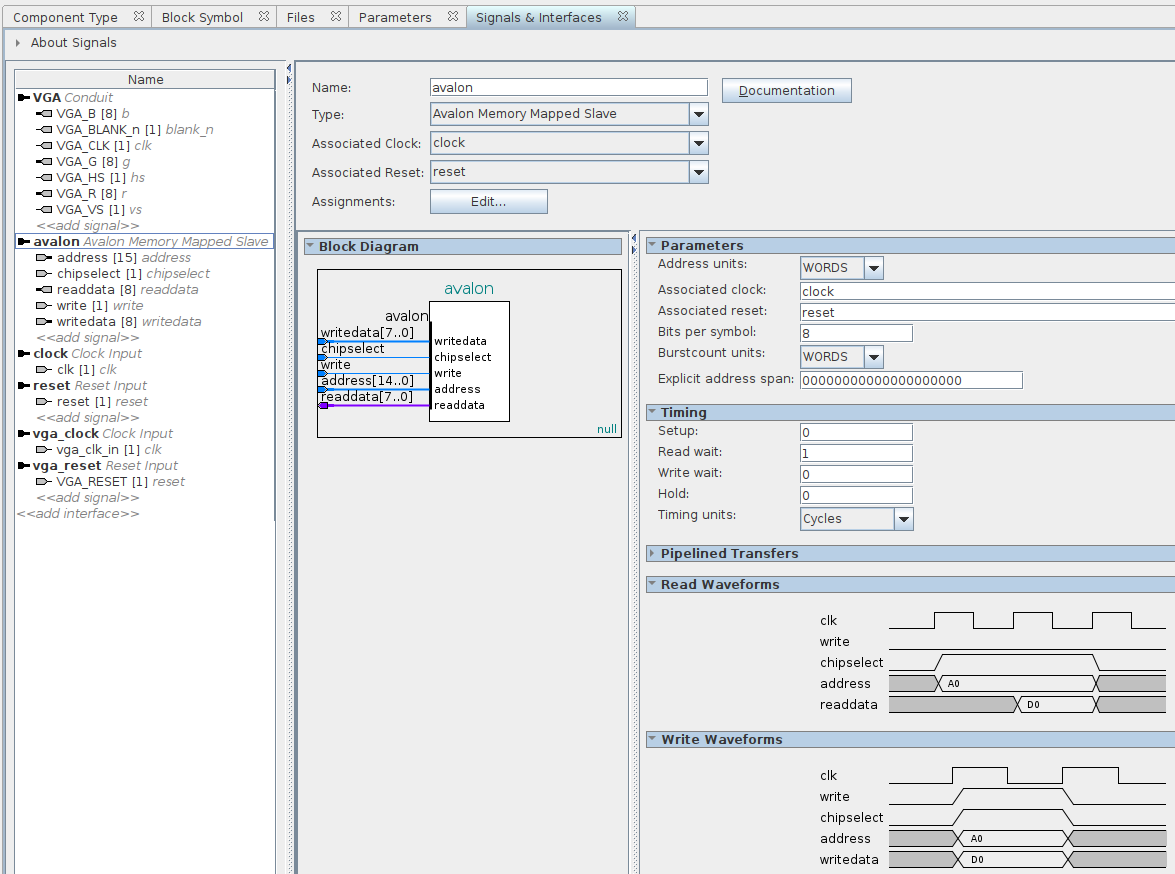
\includegraphics[width=\textwidth]{qsys-component.png}
  \caption{Signals \& Interfaces for the \emph{vga\_tiles} component.
     This shows the configuration of the Avalon MM Agent port.}
  \label{fig:qsys-component}
\end{figure}

\clearpage


% qsys-system.pdf: Play around with display in Platform Designer, then
% right-click to print (to out.ps), then ps2pdf then pdfcrop.

\begin{figure}
  \centerline{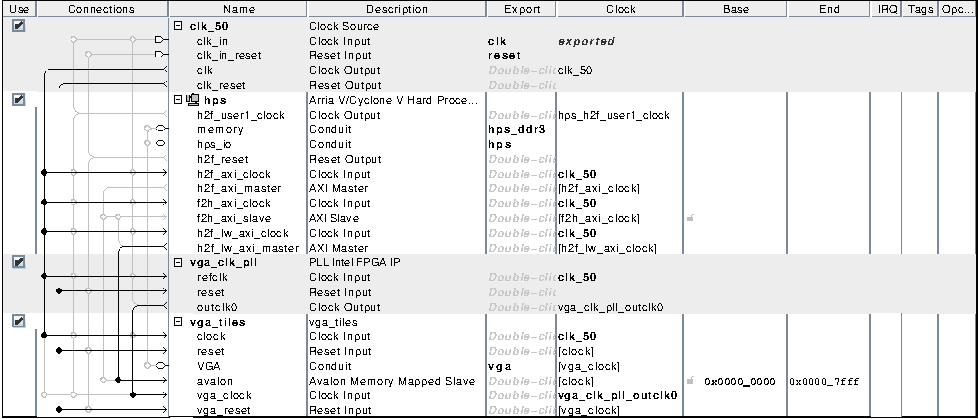
\includegraphics[width=0.9\textwidth]{qsys-system.pdf}}
  
  \vspace{-0.8\baselineskip}
  
  \caption{The Platform Designer system for the tile generator}
  \label{fig:qsys}
\end{figure}

\section{Making a Platform Designer System}

I copied the \emph{Makefile}, \emph{soc\_system.tcl},
\emph{soc\_system.qsys}, and \emph{soc\_system.srf} from Lab~3 and ran
Platform Designer (\emph{qsys-edit}).

I added \figref{vga-tiles} as an \textsc{ip} component in Platform
Designer to connect it to the \textsc{hps}.  I followed the procedure
in Lab~3: create a new \emph{vga\_tiles} component; add the
\emph{vga\_tiles.sv}, \emph{tiles.sv}, \emph{vga\_counters.sv}, and
\emph{twoportbram.sv} files; add a \emph{VGA} conduit; move and rename
the \textsc{vga} signals to it; and ensure its read wait timing was
set to~1, to allow time to read the synchronous \textsc{bram}s and its
write wait to~0 (the defaults).  \figref{qsys-component} shows the
signals.

I added the following lines to \emph{vga\_tiles\_hw.tcl} to add the
component to the device tree:

\vspace{-0.5\baselineskip}

{\footnotesize
\begin{verbatim}
set_module_assignment embeddedsw.dts.group vga
set_module_assignment embeddedsw.dts.name vga_tiles
set_module_assignment embeddedsw.dts.vendor csee4840
\end{verbatim}
}

\vspace{-0.5\baselineskip}

Unlike Lab~3, this \textsc{vga} video system runs at the \textsc{vga}
pixel clock frequency, which I generated with one of the six
phased-locked loops (\textsc{pll}s) on our \textsc{fpga}.  These are
clever digital/analog circuits that drive a voltage-controlled
oscillator from a phase detector in a feedback loop with a
programmable clock divider $M$. The reference clock passes through a
divider $N$ before going to the phase detector; the output passes
through another divider $C$.  This produces a clock whose frequency is
the reference clock's multiplied by $M \div (N \times C$), where $M$,
$N$, and $C$ are integers (1--512).  Our \textsc{fpga} has a~50~MHz
clock, and we want~25.175~MHz.  Giving Platform Designer these two
frequencies, it suggests $50\ \text{MHz} \times 215 \div (7 \times 61)
= 25.175644\ \text{MHz}$, which is close enough for a monitor.

I added the \textsc{pll} and tile components and connected them as
shown in \figref{qsys}.  Note that the \emph{refclk} for the
\textsc{pll} comes from the~50~MHz clock from the \emph{clk\_50} Clock
Source and that the \textsc{pll}'s \emph{outclk0} is sent to both the
tile component and the \emph{h2f\_lw\_axi\_clock} input: the clock for
the lightweight bus bridge on the \textsc{hps} that is connected to
the Avalon MM agent port on the Tile component.  I also exported the
\textsc{vga} conduit to make a connection.

% Fmax from soc_system.sta.rpt
% something like 121 MHz

\section{Testing the VGA Tiles Component with U-Boot}

While this component is designed to work with Linux, it is convenient
to test it separately from device drivers.  U-Boot, the first-stage
bootloader, can do this since it provides a low-level command-line
interface capable of writing to and reading from memory.

I copied the \emph{soc\_system.rbf} file over to the boot partition on
the \textsc{sd} card and started booting Linux, which starts with
loading the \emph{rbf} file to the \textsc{fpga}.  This gave a blank
display.  Before Linux started completely, I rebooted by pressing the
\emph{HPS reset} button the board and pressed a key when prompted to
\emph{Hit any key to stop autoboot}.

First, I set a base address, which is added to all address
specifications to reduce typing:

{\footnotesize 
\begin{verbatim}
SOCFPGA_CYCLONE5 # base ff200000 
Base Address: 0xff200000
\end{verbatim}
}

Three commands are convenient for reading and modifying memory:
\emph{md.b}, which displays a range of memory; \emph{mw.b}, which
writes a single byte or a range of identical bytes to memory; and
\emph{mm.b}, which modifies a range of memory by allowing you to enter
a new byte at each address.

The palette region (at offset 2000) should not change until a fourth
byte is written.  Note that in the below, the three color component
values at 2000, 2001, and 2002 are not written until 2003 is written.
This changed the screen to magenta since I modified color~0.  In the
tileset, tile~0 is all color~0, and the tilemap is all~tile~0.

{\footnotesize 
\begin{verbatim}
SOCFPGA_CYCLONE5 # md.b 2000 40 
ff202000: 00 00 00 00 00 00 00 00 00 00 00 00 00 00 00 00    ................
ff202010: 00 00 00 00 00 00 00 00 00 00 00 00 00 00 00 00    ................
ff202020: 00 00 00 00 00 00 00 00 00 00 00 00 00 00 00 00    ................
ff202030: 00 00 00 00 00 00 00 00 00 00 00 00 00 00 00 00    ................
SOCFPGA_CYCLONE5 # mw.b 2000 ff 
SOCFPGA_CYCLONE5 # md.b 2000 10
ff202000: 00 00 00 00 00 00 00 00 00 00 00 00 00 00 00 00    ................
SOCFPGA_CYCLONE5 # mw.b 2001 80 
SOCFPGA_CYCLONE5 # mw.b 2002 fe
SOCFPGA_CYCLONE5 # md.b 2000 10
ff202000: 00 00 00 00 00 00 00 00 00 00 00 00 00 00 00 00    ................
SOCFPGA_CYCLONE5 # mw.b 2003 0
SOCFPGA_CYCLONE5 # md.b 2000 10 
ff202000: ff 80 fe 00 00 00 00 00 00 00 00 00 00 00 00 00    ................
\end{verbatim}
}

\clearpage

I tested the Tilemap region (at offset 0) by writing a sequence of
``random'' bytes then verifying they could be read back.

{\footnotesize 
\begin{verbatim}
SOCFPGA_CYCLONE5 # md.b 0 10 
ff200000: 00 00 00 00 00 00 00 00 00 00 00 00 00 00 00 00    ................
SOCFPGA_CYCLONE5 # mm.b 0
ff200000: 00 ? 1
ff200001: 00 ? 5
ff200002: 00 ? 10
ff200003: 00 ? 55
ff200004: 00 ? 43
ff200005: 00 ? 72
ff200006: 00 ? aa
ff200007: 00 ? ee
ff200008: 00 ? f0
ff200009: 00 ? 0f
ff20000a: 00 ? ff
ff20000b: 00 ? 00
ff20000c: 00 ? x
SOCFPGA_CYCLONE5 # md.b 0 10
ff200000: 01 05 10 55 43 72 aa ee f0 0f ff 00 00 00 00 00    ...UCr..........
\end{verbatim}
}

I tested the Tileset region (at offset 4000) and verified only the
top~4 bits of each byte were retained:

{\footnotesize 
\begin{verbatim}
SOCFPGA_CYCLONE5 # mm.b 4000 
ff204000: 00 ? 1
ff204001: 00 ? 2
ff204002: 00 ? 4
ff204003: 00 ? 8 
ff204004: 00 ? a
ff204005: 00 ? F
ff204006: 00 ? 10
ff204007: 00 ? f0
ff204008: 00 ? ff
ff204009: 00 ? f1
ff20400a: 00 ? f3
ff20400b: 00 ? x
SOCFPGA_CYCLONE5 # md.b 4000 10
ff204000: 01 02 04 08 0a 0f 00 00 0f 01 03 00 00 00 00 00    ................
\end{verbatim}
}

\clearpage

U-Boot is able to read into memory files from the \textsc{fat}
(Microsoft) filesystem on the \textsc{sd} card.  The boot scripts do
this as part of configuring the \textsc{fpga}; it can also help test
our peripheral.  By design, the hardware uses the same data layout as
the software prototype (\figref{tile-sw}) for the tilemap, tileset,
and palette regions.  In particular, palette colors are padded to
align on~4-byte boundaries (see the software model in \figref{memmap}).

The boot partition on the \textsc{sd} card is \texttt{mmc 0:1} to
U-Boot; \emph{fatls} lists the files there:

{\footnotesize
\begin{verbatim}
SOCFPGA_CYCLONE5 # fatls mmc 0:1 
   237800   u-boot.img 
      226   u-boot.scr 
  7007204   soc_system.rbf 
    31245   soc_system.dtb 
  4877224   zimage 
       64   palette1.bin 
     8192   tilemap1.bin 
    16384   tileset1.bin
\end{verbatim}
}

U-Boot supports environment variables.  The \emph{fpgadata} variable
comes set an address to load file data.  We will set three additional
variables to the base of each region and stop using the \emph{base}
feature.

{\footnotesize
\begin{verbatim}
SOCFPGA_CYCLONE5 # tilemap=ff200000
SOCFPGA_CYCLONE5 # palette=ff202000
SOCFPGA_CYCLONE5 # tileset=ff204000
SOCFPGA_CYCLONE5 # base 0
Base Address: 0x00000000
\end{verbatim}
}

The \emph{fatload} command reads a file into memory; the \emph{cp.b}
command copies memory regions.  Using this, we can load each of the
binary files into memory, then into the peripheral:

{\footnotesize
\begin{verbatim}
SOCFPGA_CYCLONE5 # fatload mmc 0:1 $fpgadata palette1.bin 
reading palette1.bin
64 bytes read in 4 ms (15.6 KiB/s)
SOCFPGA_CYCLONE5 # cp.b $fpgadata $palette 40

SOCFPGA_CYCLONE5 # fatload mmc 0:1 $fpgadata tilemap1.bin
reading tilemap1.bin
8192 bytes read in 6 ms (1.3 MiB/s)
SOCFPGA_CYCLONE5 # cp.b $fpgadata $tilemap 2000

SOCFPGA_CYCLONE5 # fatload mmc 0:1 $fpgadata tileset1.bin
reading tileset1.bin
16384 bytes read in 5 ms (3.1 MiB/s)
SOCFPGA_CYCLONE5 # cp.b $fpgadata $tileset 4000
\end{verbatim}
}

\figref{screenshot} shows the image that appeared, which matched
\figref{tile-output}(a).

\begin{figure}
  \centerline{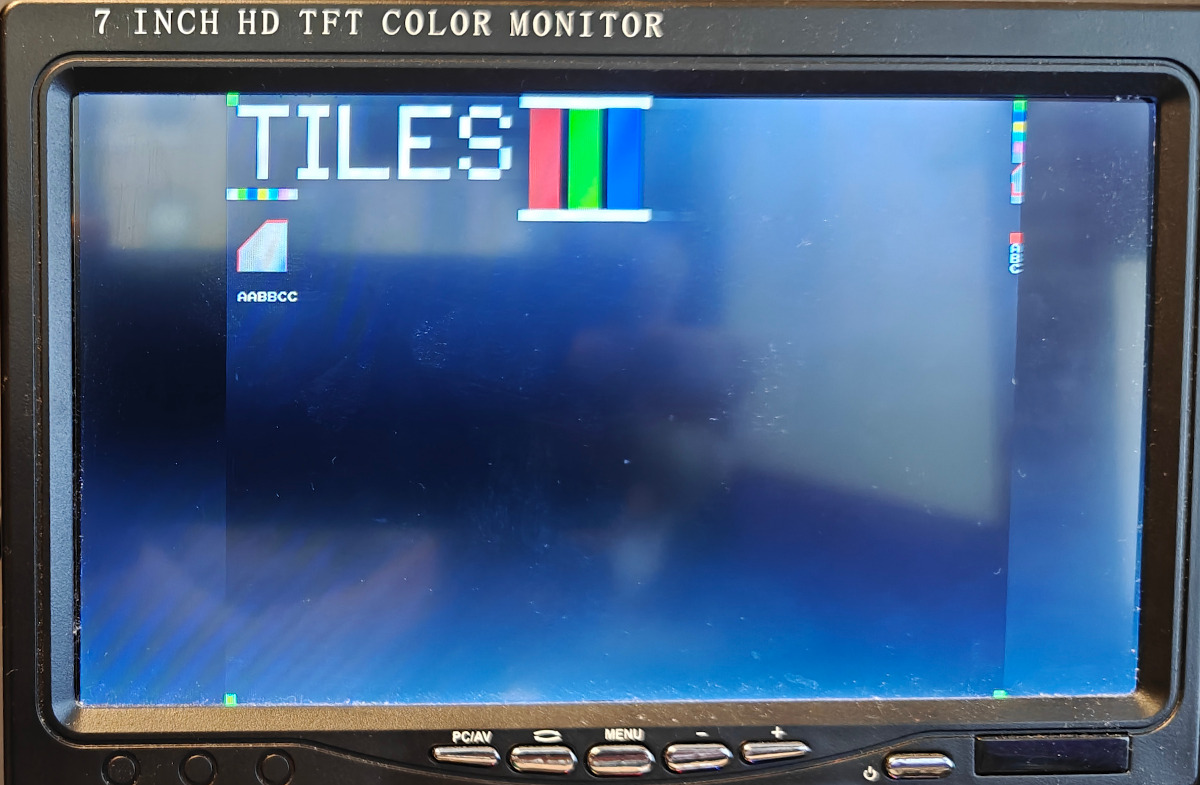
\includegraphics[width=0.75\textwidth]{screenshot.jpg}}
  \caption{The tile generator displayed on a small \textsc{vga} \textsc{lcd} monitor}
  \label{fig:screenshot}
\end{figure}

\begin{figure}
  {\footnotesize
    \begin{tabular}{ll}
  Flow Status                    & Successful - Sun May  4 20:13:58 2025       \\
 Quartus Prime Version           & 21.1.0 Build 842 10/21/2021 SJ Lite Edition \\
 Revision Name                   & soc\_system                                  \\
 Top-level Entity Name           & soc\_system\_top                              \\
 Family                          & Cyclone V                                   \\
 Device                          & 5CSEMA5F31C6                                \\
 Timing Models                   & Final                                       \\
 Logic utilization (in ALMs)     & 406 / 32,070 ( 1 \% )                        \\
 Total registers                 & 598                                         \\
 Total pins                      & 362 / 457 ( 79 \% )                          \\
 Total virtual pins              & 0                                           \\
 Total block memory bits         & 131,456 / 4,065,280 ( 3 \% )                 \\
 Total DSP Blocks                & 0 / 87 ( 0 \% )                              \\
 Total HSSI RX PCSs              & 0                                           \\
 Total HSSI PMA RX Deserializers & 0                                           \\
 Total HSSI TX PCSs              & 0                                           \\
 Total HSSI PMA TX Serializers   & 0                                           \\
 Total PLLs                      & 1 / 6 ( 17 \% )                              \\
 Total DLLs                      & 1 / 4 ( 25 \% )                              \\
  \end{tabular}}
  \caption{Quartus compilation report.  This confirms we used one
    \textsc{pll} and the three memory regions (Tilemap, Tileset, and
    Palette) were implemented with block memory ($8\text{K} \times 8 +
    16\text{K} \times 4 + 16 \times 24$).  The logic use (406
    \textsc{alm}s) was minimal.}

  \label{fig:synthesis-results}

\end{figure}



\end{document}


Test with uboot: base, mw.b, mm.b, md.b

\begin{verbatim}
SOCFPGA_CYCLONE5 # base ff200000 
Base Address: 0xff200000
SOCFPGA_CYCLONE5 # md.b 0 80 
ff200000: 00 00 00 00 00 00 00 00 00 00 00 00 00 00 00 00    ................
ff200010: 00 00 00 00 00 00 00 00 00 00 00 00 00 00 00 00    ................
ff200020: 00 00 00 00 00 00 00 00 00 00 00 00 00 00 00 00    ................
SOCFPGA_CYCLONE5 # mm.b 0 
ff200000: 00 ? 1
ff200001: 00 ? 5
ff200002: 00 ? 10
ff200003: 00 ? 55
ff200004: 00 ? 43
ff200005: 00 ? 72
ff200006: 00 ? aa
ff200007: 00 ? ee
ff200008: 00 ? f0
ff200009: 00 ? 0f
ff20000a: 00 ? ff
ff20000b: 00 ? 00
ff20000c: 00 ? x
SOCFPGA_CYCLONE5 # md.b 0 10
ff200000: 01 05 10 55 43 72 aa ee f0 0f ff 00 00 00 00 00    ...UCr..........
SOCFPGA_CYCLONE5 # mm.b 4000 
ff204000: 00 ? 1
ff204001: 00 ? 2
ff204002: 00 ? 4
ff204003: 00 ? 8 
ff204004: 00 ? a
ff204005: 00 ? F
ff204006: 00 ? 10
ff204007: 00 ? f0
ff204008: 00 ? ff
ff204009: 00 ? f1
ff20400a: 00 ? f3
ff20400b: 00 ? x
SOCFPGA_CYCLONE5 # md.b 4000 10
ff204000: 01 02 04 08 0a 0f 00 00 0f 01 03 00 00 00 00 00    ................
\end{verbatim}


Made a mistake with where the PLL was getting its clock source from, which was
generating incorrect HS and VS signals.  An oscilloscope was the tool to use.

Fixing the PLL made it display a black raster.


Utilization statistics for the final version would be helpful.

Now it's working: I can control tiles and individual pixels.

Next step: I can put tilemap and tileset binaries on the SD card and load them
with uboot.


\end{document}



SOCFPGA_CYCLONE5 # fatls mmc 0:1 
   237800   u-boot.img 
      226   u-boot.scr 
  7007204   soc_system.rbf 
    31245   soc_system.dtb 
  4877224   zimage 
       64   palette1.bin 
     8192   tilemap1.bin 
    16384   tileset1.bin   

Does not heed base address
    
fatload mmc 0:1 ff202000 palette1.bin

[    0.000000] Virtual kernel memory layout:
[    0.000000]     vector  : 0xffff0000 - 0xffff1000   (   4 kB)
[    0.000000]     fixmap  : 0xffc00000 - 0xfff00000   (3072 kB)
[    0.000000]     vmalloc : 0xf0800000 - 0xff800000   ( 240 MB)
[    0.000000]     lowmem  : 0xc0000000 - 0xf0000000   ( 768 MB)
[    0.000000]     pkmap   : 0xbfe00000 - 0xc0000000   (   2 MB)
[    0.000000]     modules : 0xbf000000 - 0xbfe00000   (  14 MB)
[    0.000000]       .text : 0x(ptrval) - 0x(ptrval)   (9184 kB)
[    0.000000]       .init : 0x(ptrval) - 0x(ptrval)   (1024 kB)
[    0.000000]       .data : 0x(ptrval) - 0x(ptrval)   ( 515 kB)
[    0.000000]        .bss : 0x(ptrval) - 0x(ptrval)   ( 135 kB)


printenv

fpgadata=0x2000000
fpgadatasize=0x700000


callscript=if fatload mmc 0:1 $fpgadata $scriptfile;then source $fpgadata; else echo Optional boot script not found. Continuing to boot normally; fi;

SOCFPGA_CYCLONE5 # fatload mmc 0:1 $fpgadata tilemap1.bin
reading tilemap1.bin 
8192 bytes read in 5 ms (1.6 MiB/s)
SOCFPGA_CYCLONE5 # md.b $fpgadata 20
02000000: 02 00 00 00 00 00 00 00 00 00 00 00 00 00 00 00    ................
02000010: 00 00 00 00 00 00 00 00 00 00 00 00 00 01 01 01    ................


SOCFPGA_CYCLONE5 # tilemap=ff200000
SOCFPGA_CYCLONE5 # palette=ff202000
SOCFPGA_CYCLONE5 # tileset=ff204000

SOCFPGA_CYCLONE5 # fatload mmc 0:1 $fpgadata palette1.bin 
reading palette1.bin
64 bytes read in 4 ms (15.6 KiB/s)
SOCFPGA_CYCLONE5 # cp.b $fpgadata $palette 40 
SOCFPGA_CYCLONE5 # md.b $palette 40 
ff202000: 00 00 00 00 ff 00 00 00 00 ff 00 00 00 00 ff ff    ................
ff202010: ff ff 00 00 00 ff ff ff ff 00 ff ff 80 80 80 80    ................
ff202020: 00 00 00 00 00 00 00 00 00 00 00 00 00 00 00 00    ................
ff202030: 00 00 00 00 00 00 00 00 00 00 00 00 ff ff ff ff    ................

OCFPGA_CYCLONE5 # fatload mmc 0:1 $fpgadata tilemap1.bin 
reading tilemap1.bin
8192 bytes read in 6 ms (1.3 MiB/s)
SOCFPGA_CYCLONE5 # cp.b $fpgadata $tilemap 2000
SOCFPGA_CYCLONE5 # md.b $tilemap 40 
ff200000: 02 00 00 00 00 00 00 00 00 00 00 00 00 00 00 00    ................
ff200010: 00 00 00 00 00 00 00 00 00 00 00 00 00 01 01 01    ................
ff200020: 01 01 01 01 01 01 01 01 01 01 00 00 00 00 00 00    ................
ff200030: 00 00 00 00 00 00 00 00 00 00 00 00 00 00 00 00    ................

SOCFPGA_CYCLONE5 # fatload mmc 0:1 $fpgadata tileset1.bin 
reading tileset1.bin
16384 bytes read in 6 ms (2.6 MiB/s)
SOCFPGA_CYCLONE5 # cp.b $fpgadata $tileset 4000


SOCFPGA_CYCLONE5 #  tilemap=ff200000
SOCFPGA_CYCLONE5 #  palette=ff202000
SOCFPGA_CYCLONE5 # tileset=ff204000
SOCFPGA_CYCLONE5 #  fatload mmc 0:1 $fpgadata palette1.bin 
reading palette1.bin
64 bytes read in 4 ms (15.6 KiB/s)
SOCFPGA_CYCLONE5 #  cp.b $fpgadata $palette 40
SOCFPGA_CYCLONE5 #  fatload mmc 0:1 $fpgadata tilemap1.bin
reading tilemap1.bin
8192 bytes read in 6 ms (1.3 MiB/s)
SOCFPGA_CYCLONE5 #  cp.b $fpgadata $tilemap 2000
SOCFPGA_CYCLONE5 #  fatload mmc 0:1 $fpgadata tileset1.bin
reading tileset1.bin
16384 bytes read in 5 ms (3.1 MiB/s)
SOCFPGA_CYCLONE5 #  cp.b $fpgadata $tileset 4000





% soc_system0|vga_clk_pll|altera_pll_i|general[0].gpll~PLL_OUTPUT_COUNTER|divclk

